\documentclass[12pt,a4paper]{article}
\usepackage[utf8]{inputenc}
\usepackage[spanish]{babel}
\usepackage{graphicx}
\usepackage{float}
\usepackage{geometry}
\usepackage{hyperref}
\usepackage{fancyhdr}
\usepackage{titlesec}
\usepackage{booktabs}
\usepackage{xcolor}
\usepackage{verbatim}
\usepackage{mathptmx}
\usepackage{setspace}
\usepackage{xurl}
\usepackage{amsmath}

\geometry{top=2.5cm, bottom=2.5cm, left=3cm, right=3cm}
\hypersetup{colorlinks=true, linkcolor=black, urlcolor=blue, citecolor=black}

\graphicspath{{../resultados/}}

\pagestyle{fancy}
\fancyhf{}
\fancyhead[L]{\small Taller Algoritmo Genetico}
\fancyhead[R]{\thepage}
\renewcommand{\headrulewidth}{0.4pt}

\titleformat{\section}{\normalfont\Large\bfseries}{\thesection}{1em}{}
\titleformat{\subsection}{\normalfont\large\bfseries}{\thesubsection}{1em}{}
\titleformat{\subsubsection}{\normalfont\normalsize\bfseries}{\thesubsubsection}{1em}{}

\begin{document}

\begin{titlepage}
\thispagestyle{empty}
\centering

\vspace*{1.5cm}

{\fontsize{13}{15}\selectfont\textbf{UNIVERSIDAD SERGIO ARBOLEDA}}\\[2.5cm]

{\fontsize{14}{17}\selectfont\textbf{TALLER: DISE\~{N}O E IMPLEMENTACI\'{O}N DE UN\\
ALGORITMO GEN\'{E}TICO}}\\[3.5cm]

{\fontsize{12}{14}\selectfont\textbf{Introducci\'{o}n a la Inteligencia Artificial}}\\[1.8cm]

{\fontsize{12}{14}\selectfont Camilo Andr\'{e}s D\'{i}az Garc\'{i}a}\\[0.3cm]

\vfill

\begin{center}
    \textit{Universidad Sergio Arboleda}\\
    \textit{Facultad de Sistemas e Ingenier\'{i}a}\\
    \textit{Bogot\'{a} D.C., 2026}
\end{center}

\end{titlepage}

\newpage
\tableofcontents
\newpage

\section{Formulaci\'{o}n del problema}

El problema consiste en seleccionar el subconjunto de diez proyectos
de innovaci\'{o}n que maximiza el beneficio total sin superar un
presupuesto de 50 unidades monetarias. Corresponde a una variante
del problema de la mochila 0/1.

\textbf{Variable de decisi\'{o}n.} Para cada proyecto $i = 1, \dots, 10$ se
define $x_i \in \{0,1\}$, donde $x_i = 1$ si el proyecto $i$ se
selecciona y $x_i = 0$ en caso contrario.

\textbf{Funci\'{o}n objetivo.} Maximizar el beneficio total:
\[
B(X) = \sum_{i=1}^{10} b_i x_i
\]

\textbf{Restricci\'{o}n principal.} El costo total no puede superar el
presupuesto disponible:
\[
C(X) = \sum_{i=1}^{10} c_i x_i \leq 50
\]

\textbf{Representaci\'{o}n de un individuo.} Cada individuo se representa
mediante un cromosoma binario de diez genes, $X = (x_1, \dots,
x_{10})$, donde cada gen indica la inclusi\'{o}n o exclusi\'{o}n del
proyecto correspondiente.

\textbf{Tama\~{n}o del espacio de b\'{u}squeda.} Existen $2^{10} = 1024$
combinaciones posibles. De estas, 587 cumplen la restricci\'{o}n de
presupuesto y las 437 restantes son inv\'{a}lidas por exceder los 50
puntos de costo.

\textbf{Ejemplo de evaluaci\'{o}n manual.} Para el individuo
$X = (1, 0, 1, 1, 0, 0, 1, 0, 1, 0)$, que selecciona los proyectos
P1, P3, P4, P7 y P9:

\[
C(X) = 12 + 11 + 8 + 6 + 5 = 42
\]
\[
B(X) = 24 + 23 + 15 + 11 + 9 = 82
\]

Como $C(X) = 42 \leq 50$, la soluci\'{o}n es v\'{a}lida.

\section{Dise\~{n}o del algoritmo gen\'{e}tico}

\begin{table}[H]
\centering
\caption{Componentes del dise\~{n}o del algoritmo gen\'{e}tico}
\label{tab:diseno}
\begin{tabular}{ll}
\toprule
\textbf{Componente} & \textbf{Dise\~{n}o adoptado} \\
\midrule
Representaci\'{o}n & Cromosoma binario de 10 genes \\
Tama\~{n}o de poblaci\'{o}n & 20 (configuraci\'{o}n inicial) \\
Funci\'{o}n de aptitud & Beneficio si $C(X) \leq 50$; penalizaci\'{o}n lineal \\
 & $B(X) - \lambda(C(X)-50)$ en caso contrario, con $\lambda = 5$ \\
Selecci\'{o}n & Torneo de tama\~{n}o 3 \\
Cruce & Un punto, probabilidad 0.80 \\
Mutaci\'{o}n & Bit-flip gen a gen, probabilidad 0.05 \\
Elitismo & Se conserva 1 individuo entre generaciones \\
Criterio de parada & N\'{u}mero fijo de generaciones (100 en la configuraci\'{o}n inicial) \\
\bottomrule
\end{tabular}
\end{table}

La penalizaci\'{o}n lineal permite que soluciones ligeramente inv\'{a}lidas
sigan participando en la selecci\'{o}n sin dominar a las soluciones
factibles, evitando as\'{i} descartar prematuramente material gen\'{e}tico
\'{u}til. Un valor de $\lambda$ demasiado peque\~{n}o deja de penalizar
efectivamente el exceso de presupuesto, favoreciendo individuos
inv\'{a}lidos; un valor demasiado grande equivale a descartar de forma
abrupta cualquier soluci\'{o}n que exceda el presupuesto, reduciendo la
diversidad disponible para la recombinaci\'{o}n.

\section{Resultados experimentales}

\subsection{Cinco ejecuciones con la configuraci\'{o}n inicial}

\begin{table}[H]
\centering
\caption{Cinco ejecuciones con la configuraci\'{o}n inicial (Punto 4)}
\label{tab:punto4}
\resizebox{\textwidth}{!}{%
\begin{tabular}{lllllll}
\toprule
\textbf{Ejec.} & \textbf{Mejor benef.} & \textbf{Costo} & \textbf{Proyectos} & \textbf{Gen. del mejor} & \textbf{Tiempo (s)} & \textbf{Apt. prom. final} \\
\midrule
1 & 97 & 50 & P1, P3, P4, P5, P8 & 1  & 0.01041 & 90.85 \\
2 & 99 & 50 & P1, P3, P4, P6, P9 & 6  & 0.00927 & 89.70 \\
3 & 99 & 50 & P1, P2, P3, P6, P7 & 10 & 0.00925 & 89.70 \\
4 & 97 & 50 & P1, P4, P6, P7, P8 & 0  & 0.00928 & 87.05 \\
5 & 99 & 50 & P1, P2, P3, P6, P7 & 11 & 0.00928 & 88.80 \\
\bottomrule
\end{tabular}%
}
\end{table}

\subsection{Experimentos A, B y C}

\begin{table}[H]
\centering
\caption{Resultados de los experimentos A, B y C (Punto 5)}
\label{tab:punto5}
\resizebox{\textwidth}{!}{%
\begin{tabular}{lllllllll}
\toprule
\textbf{Exp.} & \textbf{Pob.} & \textbf{Gen.} & \textbf{Mut.} & \textbf{Mejor benef.} & \textbf{Costo} & \textbf{Proyectos} & \textbf{Gen. del mejor} & \textbf{Tiempo (s)} \\
\midrule
A & 10 & 50  & 0.01 & 93  & 49 & P1, P5, P8, P9, P10 & 43 & 0.00255 \\
B & 20 & 100 & 0.05 & 100 & 50 & P1, P3, P6, P10     & 2  & 0.01008 \\
C & 50 & 200 & 0.10 & 100 & 50 & P1, P3, P6, P10     & 1  & 0.05027 \\
\bottomrule
\end{tabular}%
}
\end{table}

\subsection{Gr\'{a}ficas de evoluci\'{o}n}

\begin{figure}[H]
    \centering
    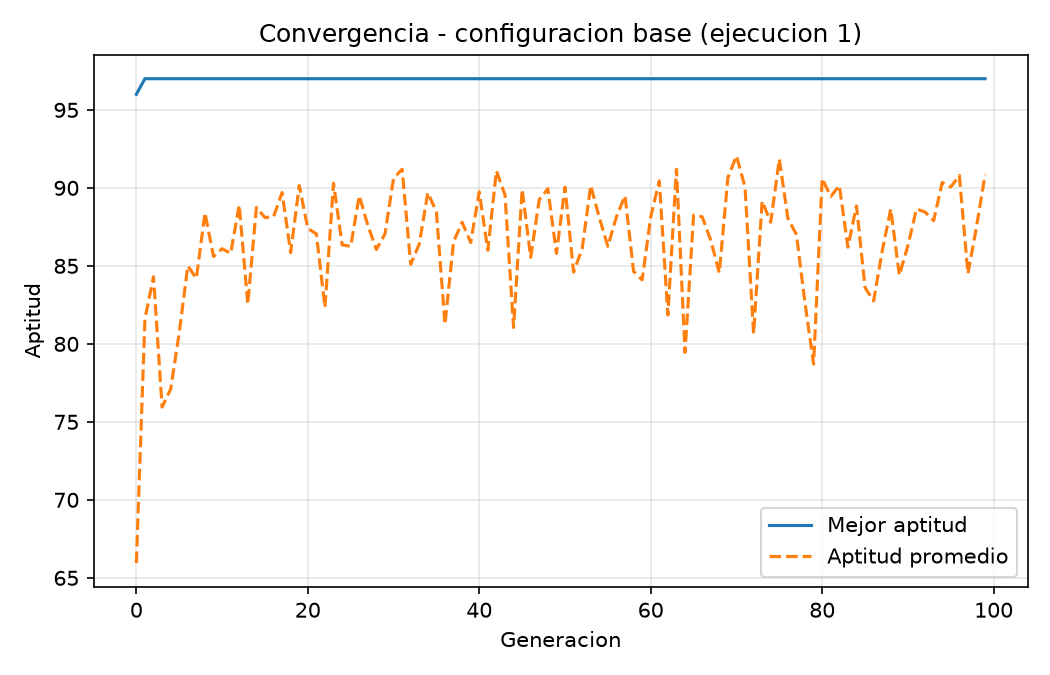
\includegraphics[width=0.85\textwidth]{convergencia_base.png}
    \caption{Convergencia de la configuraci\'{o}n base}
    \label{fig:convergencia-base}
\end{figure}

\begin{figure}[H]
    \centering
    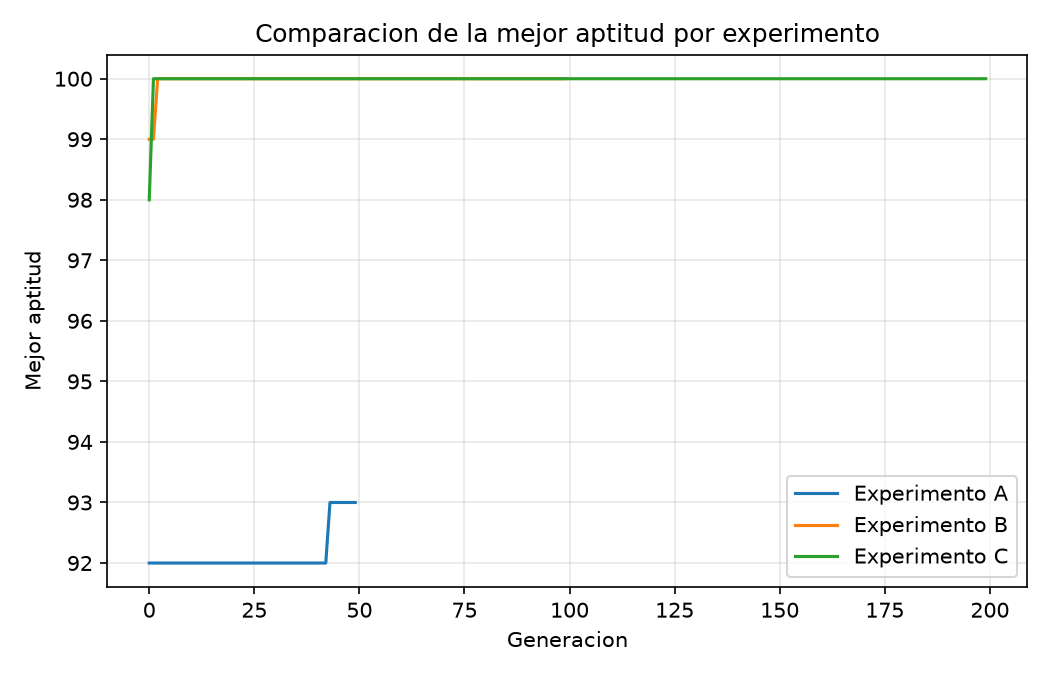
\includegraphics[width=0.85\textwidth]{comparacion_experimentos.png}
    \caption{Comparaci\'{o}n de la mejor aptitud entre experimentos}
    \label{fig:comparacion-experimentos}
\end{figure}

\section{Explicaci\'{o}n de la mejor soluci\'{o}n encontrada}

La mejor soluci\'{o}n encontrada en el conjunto de ejecuciones
corresponde al cromosoma $X = (1,0,1,0,0,1,0,0,0,1)$, que
selecciona los proyectos \textbf{P1, P3, P6 y P10}, con un costo total
de 50 unidades monetarias (exactamente el l\'{i}mite del presupuesto) y
un beneficio total de 100 unidades. Esta soluci\'{o}n fue encontrada por
los experimentos B y C, y se verific\'{o} mediante b\'{u}squeda exhaustiva
sobre las 1024 combinaciones posibles que corresponde al \'{o}ptimo
global del problema. Ninguna otra combinaci\'{o}n factible produce un
beneficio mayor.

\section{Conclusiones sobre la influencia de los par\'{a}metros}

\textbf{a) Efecto del tama\~{n}o de la poblaci\'{o}n.} Al aumentar la poblaci\'{o}n
de 10 (experimento A) a 20 y 50 individuos (experimentos B y C), el
algoritmo pas\'{o} de estancarse en un \'{o}ptimo local (beneficio 93) a
alcanzar el \'{o}ptimo global (beneficio 100) en muy pocas generaciones.
Una poblaci\'{o}n reducida limita la diversidad gen\'{e}tica inicial y
restringe el n\'{u}mero de esquemas explorados simult\'{a}neamente.

\textbf{b) Efecto de la tasa de mutaci\'{o}n sobre la diversidad.} Una tasa
de mutaci\'{o}n baja (0.01), combinada con una poblaci\'{o}n peque\~{n}a,
result\'{o} insuficiente para reintroducir diversidad una vez que la
poblaci\'{o}n convergi\'{o} hacia un conjunto reducido de soluciones. Una
tasa m\'{a}s alta (0.10) sostenida por una poblaci\'{o}n grande mantuvo
suficiente variabilidad para seguir explorando sin degradar la
convergencia.

\textbf{c) \textquestiondown Una tasa de mutaci\'{o}n alta siempre produjo mejores
resultados?} No de forma aislada. En los experimentos realizados,
la tasa de mutaci\'{o}n y el tama\~{n}o de poblaci\'{o}n variaron
simult\'{a}neamente, por lo que su efecto no puede separarse por
completo. Los resultados sugieren que una mutaci\'{o}n alta solo es
efectiva si la poblaci\'{o}n es lo suficientemente grande para sostener
la diversidad que introduce.

\textbf{d) \textquestiondown El mejor individuo apareci\'{o} antes de la \'{u}ltima generaci\'{o}n?}
S\'{i}, en todos los casos. En las cinco ejecuciones de la configuraci\'{o}n
inicial, el mejor individuo apareci\'{o} entre las generaciones 0 y 11;
en los experimentos B y C apareci\'{o} en las generaciones 2 y 1,
respectivamente. Esto es consistente con el tama\~{n}o reducido del
espacio de b\'{u}squeda del problema.

\textbf{e) \textquestiondown El algoritmo obtuvo siempre la misma soluci\'{o}n?} No. Las
cinco ejecuciones de la configuraci\'{o}n inicial obtuvieron beneficios
distintos (97, 99, 99, 97 y 99) y cromosomas distintos entre s\'{i}, lo
que evidencia la naturaleza estoc\'{a}stica del algoritmo. Solo los
experimentos con mayor poblaci\'{o}n convergieron de manera consistente
al \'{o}ptimo global.

\textbf{f) Evidencia de convergencia prematura.} En la gr\'{a}fica de
convergencia de la configuraci\'{o}n base, la mejor aptitud se
estabiliza desde la primera generaci\'{o}n y permanece constante durante
el resto de la ejecuci\'{o}n, mientras que la aptitud promedio de la
poblaci\'{o}n contin\'{u}a oscilando sin alcanzar ese valor. Esta brecha
sostenida entre el mejor individuo y el promedio poblacional es el
indicio caracter\'{i}stico de una convergencia prematura.

\textbf{g) Configuraci\'{o}n recomendada.} Se recomienda una poblaci\'{o}n de 20
a 50 individuos con una tasa de mutaci\'{o}n entre 0.05 y 0.10,
manteniendo el elitismo. Esta combinaci\'{o}n mostr\'{o} suficiente
diversidad para escapar de \'{o}ptimos locales sin sacrificar
velocidad de convergencia, dado el tama\~{n}o reducido del espacio de
b\'{u}squeda de este problema en particular.

\end{document}
